\documentclass{beamer}
\usetheme{AnnArbor}
\usecolortheme{beaver}
\usepackage[utf8]{inputenc}
\usepackage[T1]{fontenc}
\usepackage[italian]{babel}
\usepackage{soul}
\usepackage{graphicx}
\usepackage{algorithm2e}

\usepackage{fancyvrb}
\definecolor{felinesrcbgcolor}{rgb}{1,1,0.85}
\definecolor{felinesrcbgcolor}{rgb}{0.94,0.97,1}
\definecolor{felineframe}{rgb}{0.79,0.88,1}
\definecolor{myorange}{rgb}{1,0.375,0}
\fvset{frame=lines,
  framesep=3mm,
  framerule=3pt,
  fontsize=\small,
  rulecolor=\color{myorange},
  formatcom=\color{DarkGreen},
}

\hypersetup{
	urlcolor=myorange
}

\title[Arch2013] % (optional, only for long titles)
{Architettura degli elaboratori 2012/2013}
\subtitle{Rappresentazione ed aritmetica binaria di base}
\author{Michele ``Jazzinghen'' Bianchi\inst{1}}
\institute[DISI] % (optional)
{
  \inst{1}%
  Dipartimento di Ingegneria e Scienze dell'Informazione\\
  Universtià degli Studi di Trento
}
\date[FEB 2013] % (optional)
{21 Febbraio 2013}
\subject{Computer Science, Embedded Systems}

\begin{document}
	\frame{\titlepage}
	\section{Intro}
	\begin{frame}
    \frametitle{Introduzione}
		\begin{itemize}
			\item Contatti: \url{michele.bianchi@unitn.it}
		  \item Sito web con i materiali: \url{http://disi.unitn.it/~bianchi}
		  \item Ricevimento: scrivetemi una mail, così ci mettiamo d'accordo.
		  \item Domande o parti poco chiare: Ovviamente sono qui per questo, quindi
		    chiedete pure, altrimenti mandatemi le domande via mail, alle quali
		    risponderò all'inizio della lezione successiva
		\end{itemize}    
   
  \end{frame}
  \begin{frame}
    \frametitle{Introduzione}
    \framesubtitle{Extra}
    \begin{itemize}
    		\item Sulla mia pagina è presente una Quick Start Guide per quanto riguarda
    			la seconda parte del corso. Vi potrebbe essere utile leggerla subito, così
    			se ci sono casini metto a posto
    		\item Aggiungerò dei link a delle risorse online utili per il corso, dateci
    			un'occhiata ogni tanto. So che vi sentite dire questa cosa spesso, ma \st{a me%
    			servono hit per prendere soldi} nel mio caso vi potrebbe essere utile, visto
    			che non ci sono ancora tutti i contenuti.
    \end{itemize}
  \end{frame}

  \section[AllYourBases...]{Sistemi numerici (Basi)}
	\subsection{Storia della rappresentazione numerica}  
  \begin{frame}
    \frametitle{Storia}
    \begin{itemize}
    		\item Sistemi unari (dita, tacche, ideogrammi)
    		\item Sistemi di numerazione additivi (Romani, Egizi)
    		\item Sistemi letterali (e.g. \emph{Sixty nine}, \emph{Soixante dix-neuf}, \emph{Settantanove})
    		\item Notazioni posizionali (Babilonesi [base60], Hindu-Arabic [base10])
    \end{itemize}
    %Unari, Babilonesi, Romani, Posizioniali (indiani), Binaria
  \end{frame}
	
	\subsection{Basi numeriche informatiche}
  \begin{frame}
    \frametitle{Basi informatiche}
    \begin{itemize}
    		\item Base-2 (Binario): rappresentazione grezza delle linee logiche
    		\item Base-8 (Ottale): rappresentazione di 3 bit (deprecato)
    		\item Base-16 (Esadecimale): rappresentazione 4 bit (e.g. Colori per CSS)
    \end{itemize}
  \end{frame}

	\section[BinaryData]{Rappresentazione Binaria dei dati}
	\subsection{Rappresentazioni di base}  
  \begin{frame}
    \frametitle{Definizioni di base}    	
    \begin{itemize}
    		\item Bit [0,1]: stato di una linea logica
    		\item Byte [0,255]: 8 bit assieme (e.g. 1 carattere ASCII)
    		\item Word [0,$2^{bits}-1$]: numero variabile di byte a seconda del sistema (e.g. float da 4byte)
    \end{itemize}
  \end{frame}
  \subsection{Standard Types}
  \begin{frame}   	
    \begin{itemize}
    		\item Integer (8, 16, 32, 64 bit)
    			\begin{itemize}
    				\item Unsigned: Da 0 a $2^{bit}-1$
    				\item Signed: Da $-2^{bit-1}$ a $2^{bit-1}-1$
    			\end{itemize}
    		\item Float
    			\begin{itemize}
    				\item Single: $1.175494351e^{-38}$ a $3.402823466e^{38}$
    				\item Double: $2.2250738585072014e^{-308}$ a $1.7976931348623158e^{308}$
    				\item Quad (There is no kill like overkill): $3.362e^{-4932}$ a $1.20e^{4932}$
    			\end{itemize}
    \end{itemize}

		\begin{block}{N.B.}
			Per iniziare lavoreremo con i numeri naturali (interi positivi) a 8 bit. Ovvero da 0 a 255,
			come se stessimo giocando a Final Fantasy VII.
		\end{block}
    %Parlare dei vari tipi, aggiungere i limiti e dire che lavoreremo con gli unsigned.
  \end{frame}
  \subsection{Strutture dati complesse}
  \begin{frame}
    \frametitle{Strutture complesse}
    \begin{itemize}
    		\item Testo: Sequenza di byte o, nel caso di sistemi moderni, di word da 8 a 32 bit (UTF-8)
    		\item Immagini: Bitmap a profondità variabile (1, 8, 16, 24, 32 bit)
    			\begin{itemize}
    				\item 1 bit: Bianco e Nero
    				\item 8 bit: 256 colori (NES! MSX2! :D Glorious Retrogaming)
    				\item 16 bit: 65536 colori (SNES, Windows 95)
    				\item 24 bit: 16 milioni di colori (Circa tutto adesso)
    				\item 32 bit: 16 milioni di colori + Alpha Channel
    			\end{itemize}
    		\item Audio: Dati stereo codificati tramite Pulse Code Modulation (PCM)\footnote{Dannato PCM!}
    \end{itemize}
  \end{frame} 
  
  \section[Conversion]{Conversione di Base}
  \subsection{Metodi di conversione base-2 a base-10}
  \begin{frame}
  		\frametitle{Conversione base-10 a base-2}
    \framesubtitle{Valore di un numero base-10}
  		Un numero in base-10 è formato da unità, decine, centinaia, migl... blah blah.
  		
  		In pratica è la somma di multipli di potenze di 10, partendo da $10^0 = 1$
  		
  		Quindi, se prendiamo un numero tipo il $85500164_{10}$ avremo:
  		
  		\vspace{2em}
  		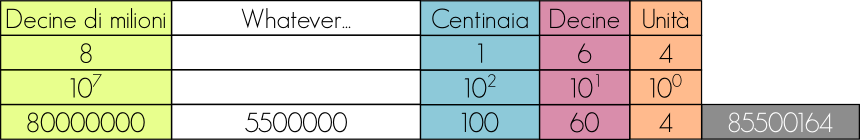
\includegraphics[width=\textwidth]{IMGs/base-10read.png}
    
  \end{frame}
  \begin{frame}
  		\frametitle{Conversione base-10 a base-2}
    \framesubtitle{Valore di un numero base-2}
  		Alla stessa maniera un numero base-2 è formato da unità, due, quattro, otto ed avanti così
  		per potenze di 2.
		
		La conversione, quindi, da base-2 a base-10 è molto semplice, basta sommare le
		potenze di 2 rappresentate dagli 1 e avremo così il numero in base-10.  		
  		
  		\vspace{2em}
  		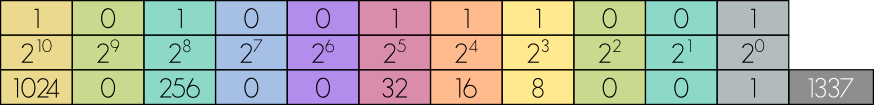
\includegraphics[width=\textwidth]{IMGs/base-2read.png}
    
  \end{frame}
  \subsection{Metodi di conversione base-10 a base-2}
	\begin{frame}
    \frametitle{Conversione base-10 a base-2}
    Ci sono due metodi per farlo:
    \begin{itemize}
    		\item \emph{Divisione e Modulo}: Continuare a dividere per due e mantenere il resto
    		\item \emph{Sottrazione}: Testare se il numero è contenuto in un multiplo di due, se sì ve
    			lo segnate da parte e poi lo sottraete dal numero e continuate così
    \end{itemize}
  \end{frame}
  \begin{frame}
    \frametitle{Conversione base-10 a base-2}
    \framesubtitle{Divisione e modulo}
    \begin{itemize}
    		\item Più facilmente implementabile
    \end{itemize}
    \begin{columns}
    \column{.6\textwidth}
    \footnotesize{
    \begin{algorithm}[H]
    		\SetAlgoLined
			 \KwData{n: Numero base-10 da convertire}
			 \KwResult{s: Numero convertito in base-2}
			 s = stringa vuota\;			 
			 \While{n>0}{
			  s = (n mod 2) + s\; 
			  n = n div 2\;
			 }
    \end{algorithm}
		}
	  \column{.4\textwidth}
	 	\footnotesize{		
			\pause
	 		$$97_{10} = ??$$
		  \pause
			\begin{tabular}{|c|l|}
			\hline
			 n & s \\
			\hline
	     97 & \\
	     48 & 1 \\
	     24 & 01 \\
	     12 & 001 \\
	     6 & 0001 \\
	     3 & 00001 \\
	     1 & 100001 \\
	     0 & 1100001 \\
			\hline
			\end{tabular}
		  $$97_{10} = 1100001_{2}$$ 
		}		
	  \end{columns}
		
		
  \end{frame}
  \begin{frame}
    \frametitle{Conversione base-10 a base-2}
    \framesubtitle{Sottrazione}
    \begin{itemize}
    		\item Terribile se usato con numeri grandi
    \end{itemize}
	\begin{columns}
  \column{.6\textwidth}
    \footnotesize{
    \begin{algorithm}[H]
    		\SetAlgoLined
			 \KwData{n: Numero base-10 da convertire}
			 \KwResult{s: Numero convertito in base-2}
			 s = stringa vuota\;
			 i = massima potenza di due contenuta in n\;		 
			 \Repeat{i=0}{
			  \eIf{$i \leq n$}{
			  		s = s + ``1''\; 
			  		n = n - i\;
			 }{
			 		s = s + ``0''\;
			 }
			  i = i div 2\;
			 }
    \end{algorithm}
	}
  \column{.4\textwidth}
 	\footnotesize{		
		\pause
 		$$117_{10} = ??$$
	  \pause
		\begin{tabular}{|c|c|l|}
		\hline
		 n & i & s \\
		\hline
     117 & 64 & \\
     53 & 32 & 1 \\
     21 & 16 & 11 \\
     5 & 8 & 111 \\
     5 & 4 & 1110 \\
     1 & 2 & 11101 \\
     1 & 1 & 111010 \\
     0 & 0 & 1110101 \\
		\hline
		\end{tabular}
	  $$117_{10} = 1110101_{2}$$ 
	}		
  \end{columns}
  \end{frame}
  
  \section[Operations]{Aritmetica dei naturali}
	\subsection[NatSum]{Somma di Naturali}  
	  \begin{frame}
	    \frametitle{Somma di naturali}
	    \framesubtitle{Un'introduzione, prima}
			\begin{center}
	    \begin{tabular}{|c|c|c||c|c|}
	    		\hline
	    			A & B & Carry & C & Carry \\
	    		\hline
	    			0 & 0 & 0 & 0 & 0 \\
	    			1 & 0 & 0 & 1 & 0 \\
	    			0 & 1 & 0 & 1 & 0 \\
	    			1 & 1 & 0 & 0 & 1 \\
	    			0 & 0 & 1 & 1 & 0 \\
	    			1 & 0 & 1 & 0 & 1 \\
	    			0 & 1 & 1 & 0 & 1 \\
	    			1 & 1 & 1 & 1 & 1 \\
	    		\hline
	    \end{tabular}
	    
	    \vspace{2em}
	    
	    A + B + Carry = C + Carry
	    \end{center}	  
	  \end{frame}
	  \begin{frame}
	    \frametitle{Somma di naturali}
	    \framesubtitle{Esempio}
	    $$117_{10} + 97_{10} = 1110101_{2} + 1100001_{2} = \text{?}$$
	    \vspace{2em}
	    \pause
			\begin{center}
			\begin{tabular}{cccccccc|c} 
			 & 1 & 1 & 1 & 0 & 1 & 0 & 1 & + \\  
			 & 1 & 1 & 0 & 0 & 0 & 0 & 1 & = \\ 
			\hline 
			1 & 1 & 0 & 1 & 0 & 1 & 1 & 0 &  \\ 
			\end{tabular}
			\end{center}
			\pause
			\vspace{2em}
			$$11010110_{2} = 214_{10}$$
	  \end{frame}
  \subsection[NatSub]{Sottrazione di Naturali}  
	  \begin{frame}
	    \frametitle{Sottrazione di naturali}
	    \framesubtitle{Operazione di base e ``Il prestito''}
	    Come nella somma si va da destra a sinistra seguendo delle regole banali:
			
			\vspace{2em}	    
	    
	    \begin{center}
		    \begin{tabular}{|c||c|c|c|c|}
		    \hline 
		    A & 0 & 1 & 1 & \textbf{0} \\ 
		    \hline 
		    B & 0 & 0 & 1 & \textbf{1} \\ 
		    \hline 
		    A-B & 0 & 1 & 0 & \textbf{1} \\ 
		    \hline 
		    \end{tabular}
	    \end{center}
	    
	    \vspace{2em}
	    
	    Nell'ultimo caso bisogna scorrere a sinistra finchè
	    non si trova un 1, invertendo il valore di tutte le cifre incontrate, 1 compreso.
	    
	    $$ 10..0 \rightarrow 01..1 $$
	  \end{frame}
	  \begin{frame}
	    \frametitle{Sottrazione di naturali}
	    \framesubtitle{Esempio}
	    $$214_{10} - 117_{10} = 11010110_{2} - 1110101_{2} = \text{?}$$
	    \vspace{2em}
	    \pause
			\begin{center}
			\begin{tabular}{cccccccc|c} 
				1 & 1 & 0 & 1 & 0 & 1 & 1 & 0 &	- \\		 
			 		& 1 & 1 & 1 & 0 & 1 & 0 & 1 & = \\  
			\hline			 
			 & 1 & 1 & 0 & 0 & 0 & 0 & 1 &  \\ 
			\end{tabular}
			\end{center}
			\pause
			\vspace{2em}
			$$1100001_{2} = 97_{10}$$
	  \end{frame}
	\subsection[NatMul]{Moltiplicazione di Naturali}  
	  \begin{frame}
	    \frametitle{Moltiplicazione di naturali}
	    \framesubtitle{Moltiplicazione (e divisione) per potenze di due}
	    Ok, se dobbiamo moltiplicare un numero base-10 per 10 dobbiamo...
	    
	    \pause
	    
	    \begin{center}
		    Aggiungere uno 0 a destra.
		    
		    
\includegraphics[width=.5\textwidth]{IMGs/youdontsay.png}
	    \end{center}
	    
	  \end{frame}
	  \begin{frame}
	    \frametitle{Moltiplicazione di naturali}
	    \framesubtitle{Moltiplicazione (e divisione) per potenze di due, cont.}
	    Nel caso dei numeri base-2, aggiungere uno 0 a destra significa
	    moltiplicare il numero per 2, mentre eliminando la prima cifra a
	    desra significa dividere per 2.
	    
	    \vspace{2em}
	    
	    Questa operazione è chiamata shifting, utilizzata spesso dai compilatori
	    per ottimizzare la moltiplicazione.
	  \end{frame}
	  \begin{frame}
	    \frametitle{Moltiplicazione di naturali}
	    \framesubtitle{Moltiplicazione tra due Naturali}
	    Moltiplicare due numeri base-2 naturali altro non è che l'applicazione
	    di shifting multipli e poi della somma sui risultati degli shifting.
	    
	    \vspace{2em}
	    
	    Alla fine non è differente dalla moltiplicazione in base-10, solo che è più
	    semplice perché o bisogna sommare uno dei due moltiplicatori shiftati o nulla.
	  \end{frame}
		\begin{frame}
	    \frametitle{Moltiplicazione di naturali}
	    \framesubtitle{Esempio}
			
			$$13_{10} x 17_{10} = 1101_{2} x 10001_{2} = \text{?}$$
	    \vspace{1em}
	    \pause	    
	    \begin{center}
	    \begin{tabular}{cccccccc||c}
	      &   &   &   & 1 & 1 & 0 & 1 & x \\ 
	      &   &   & 1 & 0 & 0 & 0 & 1 & = \\ 
	    \hline 
	      &   &   &   & 1 & 1 & 0 & 1 &  + \\ 
	      &   &   &   &   &   & - &   &  + \\ 
	      &   &   &   &   & - &   &   &  + \\ 
	      &   &   &   & - &   &   &   &  + \\ 
	    1 & 1 & 0 & 1 &   &   &   &   &   \\ 
	    \hline 
	    1 & 1 & 0 & 1 & 1 & 1 & 0 & 1 &   \\ 
	    \end{tabular} 
	    \end{center}
	    
	    \pause
			\vspace{1em}
			$$11011101_{2} = 221_{10}$$
	  \end{frame}
	\subsection[Errors]{Error checking}
		\begin{frame}
	    \frametitle{Error Checking}
	    \framesubtitle{Overflow/Underflow}
	    \begin{columns}
			\column{.6\textwidth}	    
			\footnotesize{
	    Fino ad ora abbiamo sempre fatto calcoli pensando di avere cifre infinite a nostra disposizone.
    
	    ...
	    
	    Purtroppo, la realtà ci impone dei limiti di spazio, dettati
	    dall'architettura di basso livello del calcolatore.
	    
	    A causa di questo si possono rischiare errori da semplicemente stupidi a catastrofici.
	    
	    \vspace{1em}
	    \pause
	    
	    Tipo quello che è successo all'Ariane 5 501, missile Geostationary Transfer Orbit (GTO), progettato
	    dalla Astrium per l'ESA. A causa di un errore di conversione e di mancato controllo degli Overflow
	    la casa di produzione ha bruciato 370M\$ in circa 40 secondi.
	    }
	    \column{.4\textwidth}
	    \begin{center}
	    		
\includegraphics[width=.9\textwidth]{IMGs/overflow.jpeg}
	    \end{center}
	    \end{columns}
	  \end{frame}
	  
	\begin{frame}
    \frametitle{Error Checking}
    \framesubtitle{Overflow/Underflow cont.}
    Possiamo immaginare i numeri in base-2 con una quantità limitata di cifre come se fossero posti
    intorno ad una ruota:
    
    \begin{center}
    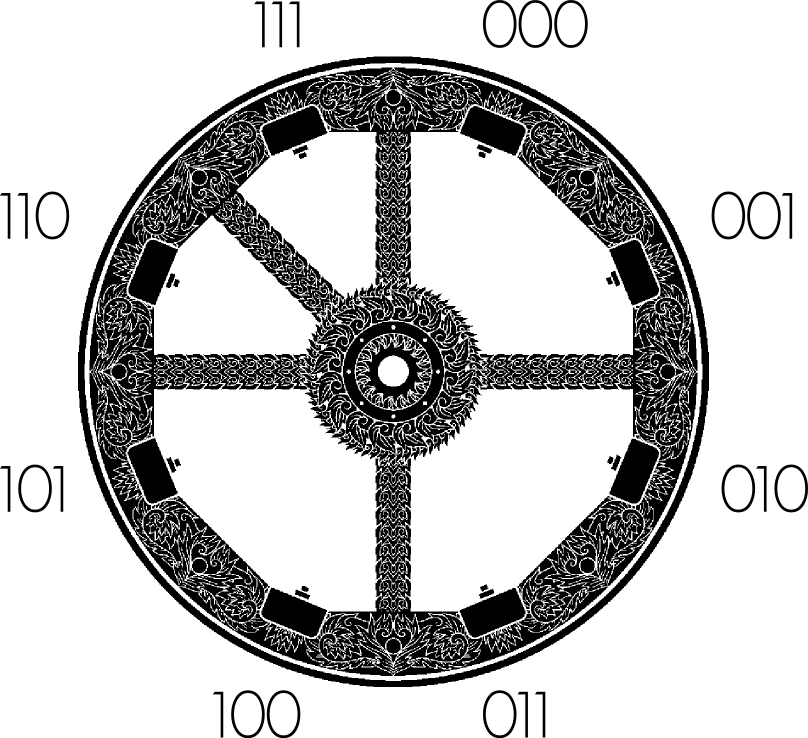
\includegraphics[width=.5\textwidth]{IMGs/TheBurningWheel.png}
    \end{center}

  \end{frame}
  
  	\begin{frame}
    \frametitle{Error Checking}
    \framesubtitle{Overflow/Underflow cont.}
    Nel caso precedente il numero è formato al massimo da 3 cifre binarie, quindi, se noi provassimo a
    calcolare $111_{2} + 1_{2}$ il risultato dovrebbe essere $1000_{2}$, solo che non abbiamo abbastanza
    cifre per contenere tutte le informazioni.
    
    Il risultato sarà quindi $000_{2}$. In pratica, $7_{10} + 1_{10} = 0_{10}$.
    
    \vspace{2em}
    \pause
    
    Fortunatamente le ALU contengono delle flag che indicano se è avvenuto un overflow (o un underflow)
    durante un'operazione aritmetica.
  \end{frame}
  
  \section[NegativeRep]{Aggiunta del segno negli interi}
  \begin{frame}
  		\frametitle{Aggiungere il segno agli interi}
  		Il supporto per i numeri negativi è stato aggiunto in vari modi\footnote{I quali dimezzano il
  		numero massimo rappresentabile}:
    \begin{itemize}
    		\item \emph{Segno-e-Modulo}: Un bit fa da segno, gli altri sono il valore del numero
    		\item \emph{Complemento ad 1}: Per avere il numero negativo invertiamo tutti i bit.
    		\item \emph{Complemento a 2}: Facciamo il complemento ad 1 e poi sommiamo 1.
    \end{itemize}
  \end{frame}
  \subsection{Segno-e-Modulo}
  \begin{frame}
  		\frametitle{Aggiungere il segno agli interi}
    \framesubtitle{Rappresentazione in Segno-e-Modulo}
    
    \begin{itemize}
    		\item Più vicino (Anzi, esattamente IL) al metodo usato per la rappresentazione dei negativi nei float
    		\item Permette l'esistenza di due 0: $+0$ e $-0$
    		\item Richiede una logica più complessa per venir implementato.
    \end{itemize}
  \end{frame}
  \subsection{Complemento a 2}
  \begin{frame}
  		\frametitle{Aggiungere il segno agli interi}
    \framesubtitle{Complemento a 2}
		Il complemento ad 1 è migliore del Segno-e-Modulo per gli interi, ma ha ancora dei problemi, tipo
		il doppio $0$ oppure il fatto che è macchinoso a causa dell'offset di $-1$ dei numeri negativi.
		
		Per questo è stato inventato il complemento a 2:
		
		\begin{itemize}
			\item Solo uno 0
			\item Trasparente per somma, sottrazione e moltiplicazione
			\item Per questo molto più facilmente implementabile a livello hardware
		\end{itemize}		    
    %Complemento ad 1 sarebbe figo, ma ci sega un valore. Complemento a 2 (Cmpl1 + 1) rimuove il problema. 
  \end{frame}
% etc
\end{document}
